Cette partie présente les diagrammes UML pour les mini-jeux exposés dans la seconde partie.

\listoffigures

\clearpage
%% Pacman

\begin{figure}[h]
 \centering
 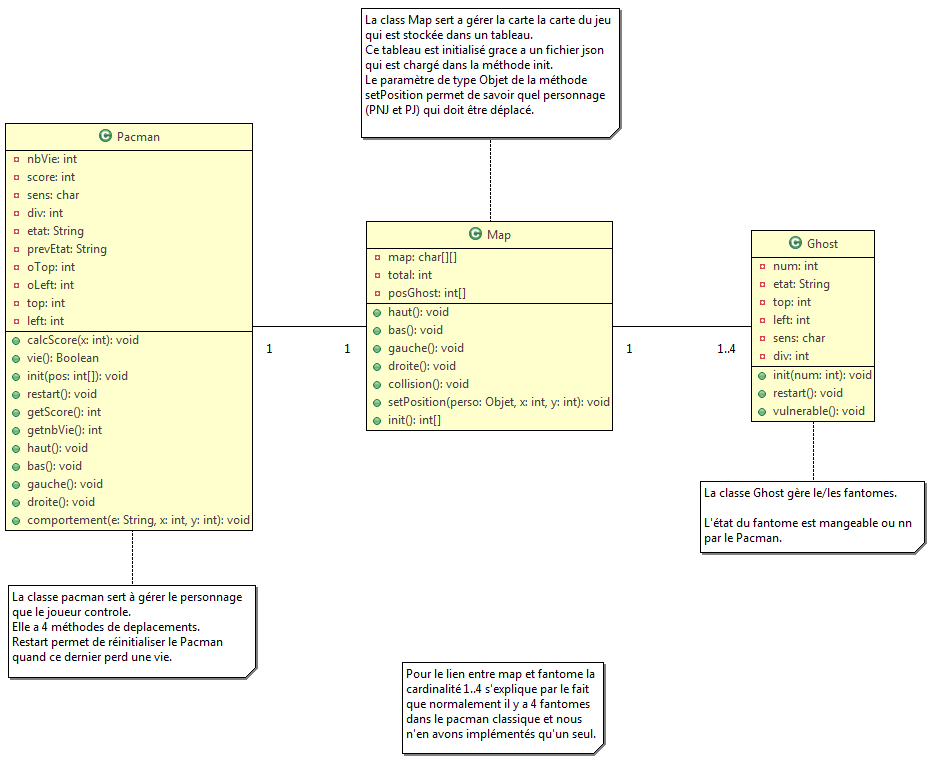
\includegraphics[width=\textwidth]{../umls/UML_images/Pacman/class} \hfill
 \caption{Pacman : Diagramme de classes}
\end{figure}

\begin{figure}[h]
 \centering
 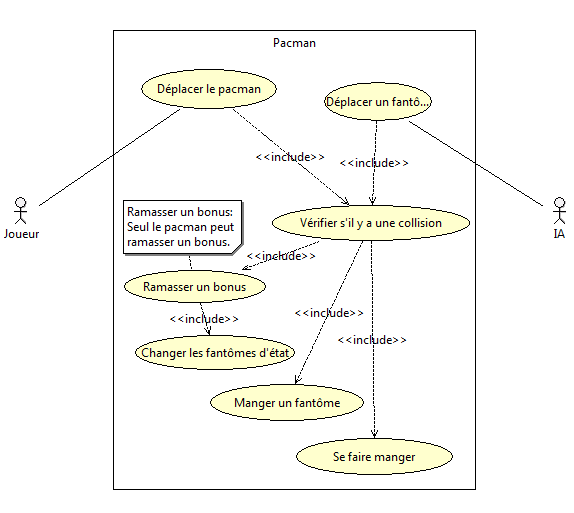
\includegraphics[width=10cm]{../umls/UML_images/Pacman/utilisation}
 \caption{Pacman : Diagramme de cas d'utilisation}
\end{figure}

\begin{figure}[h]
 \centering
 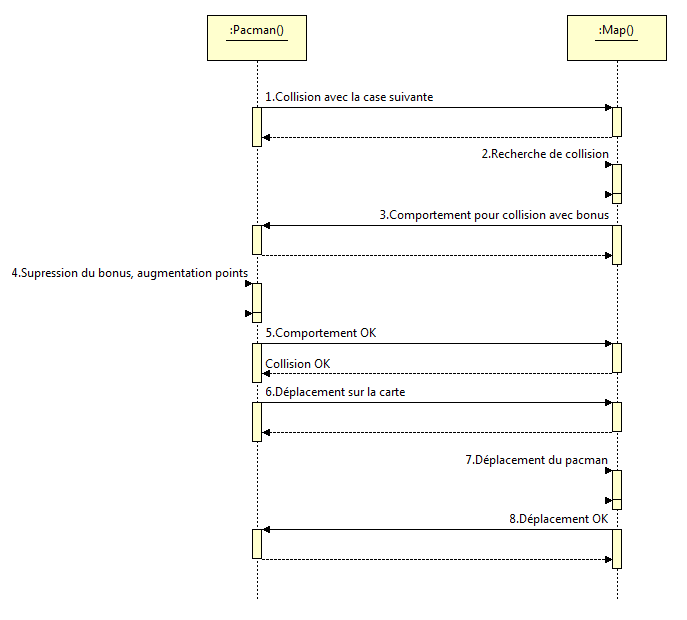
\includegraphics[width=9cm]{../umls/UML_images/Pacman/sequence} \hfill
 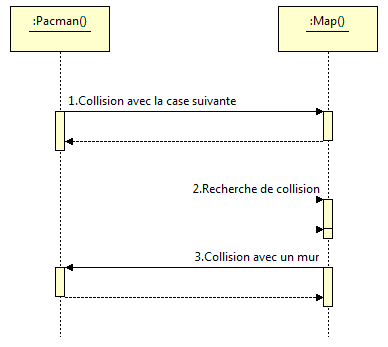
\includegraphics[width=6cm]{../umls/UML_images/Pacman/sequence2} \hfill
 \caption{Pacman : Diagrammes de séquences}
\end{figure}


\clearpage
%% 1942

\begin{figure}[h]
 \centering
 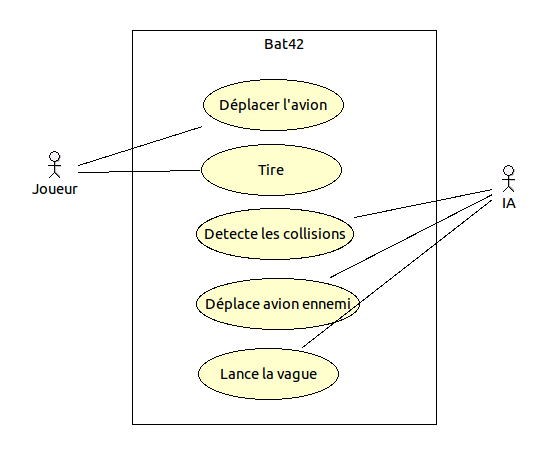
\includegraphics[height=6cm]{../umls/UML_images/Bat42/utilisation} \hfill
 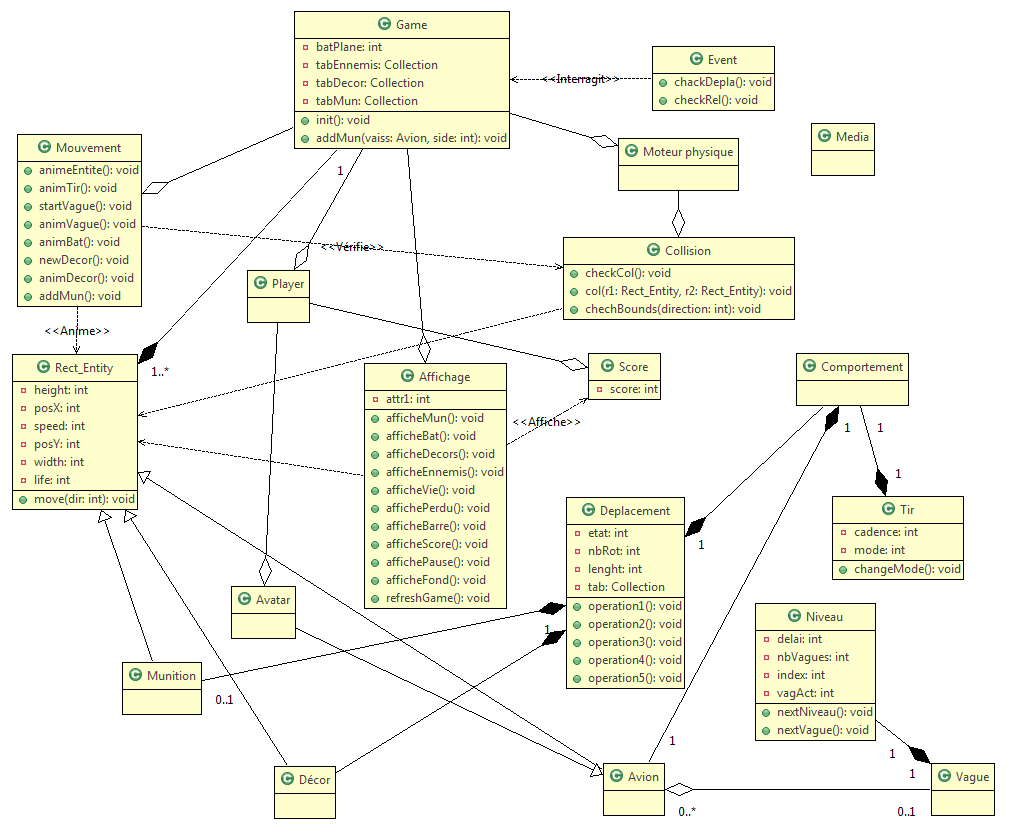
\includegraphics[height=13cm]{../umls/UML_images/Bat42/class} \hfill
 \caption{1942 : En haut, diagramme des cas d'utilisation  ; en bas, diagramme de classes}
\end{figure}

\begin{figure}[h]
 \centering
 \includegraphics[height=8cm]{../umls/UML_images/Bat42/sequence} \hfill
 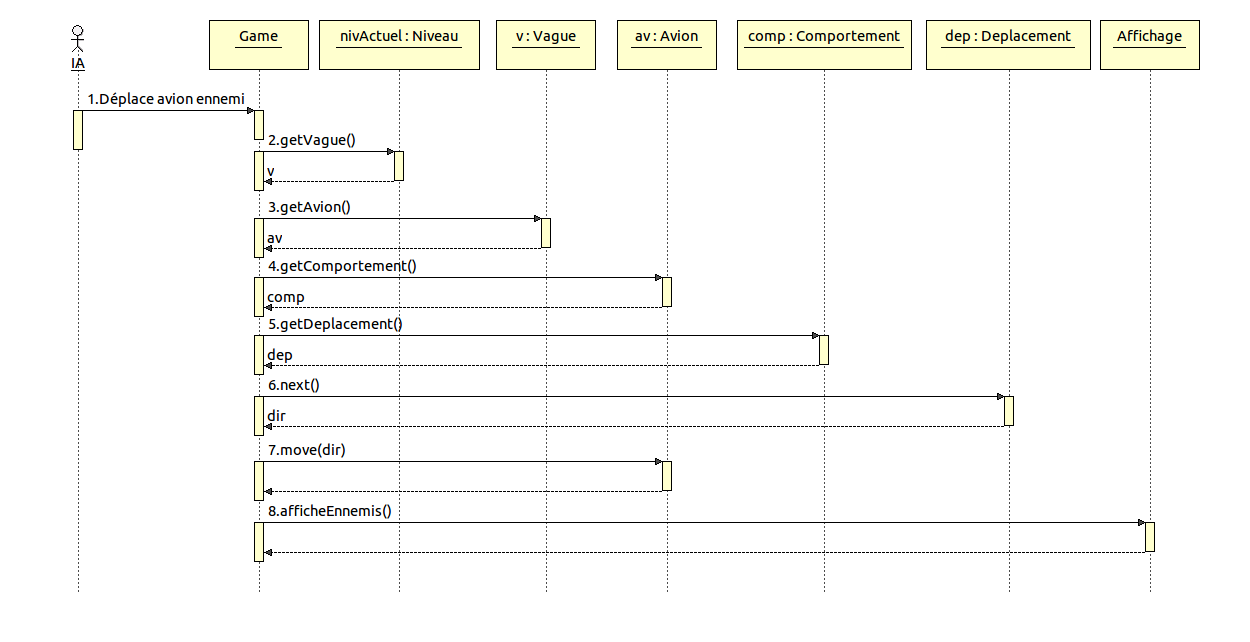
\includegraphics[width=\textwidth]{../umls/UML_images/Bat42/sequenceIA} \hfill
 \caption{1942 : Diagrammes de séquences}
\end{figure}

\clearpage
%% Volley

\begin{figure}[h]
 \centering
 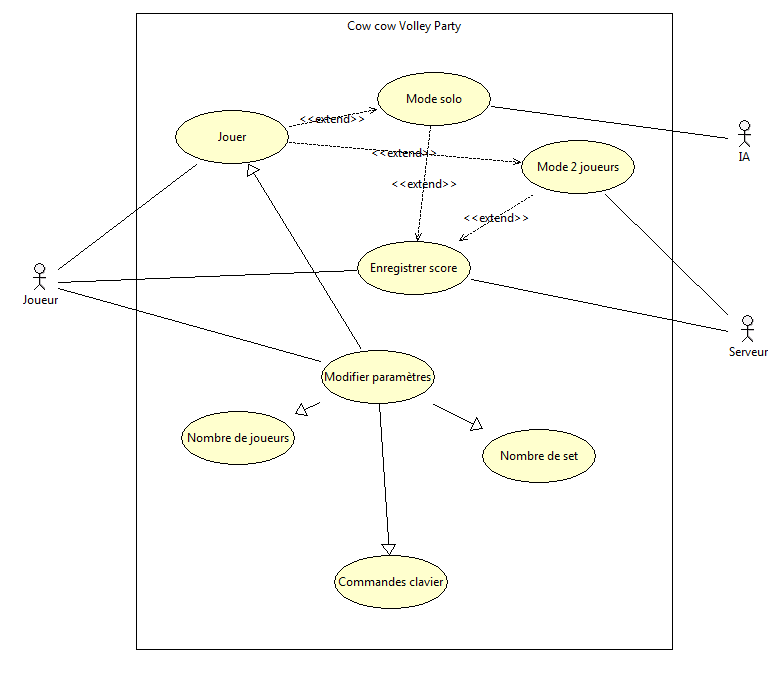
\includegraphics[height=8.5cm]{../umls/UML_images/Volley/utilisation} \hfill
 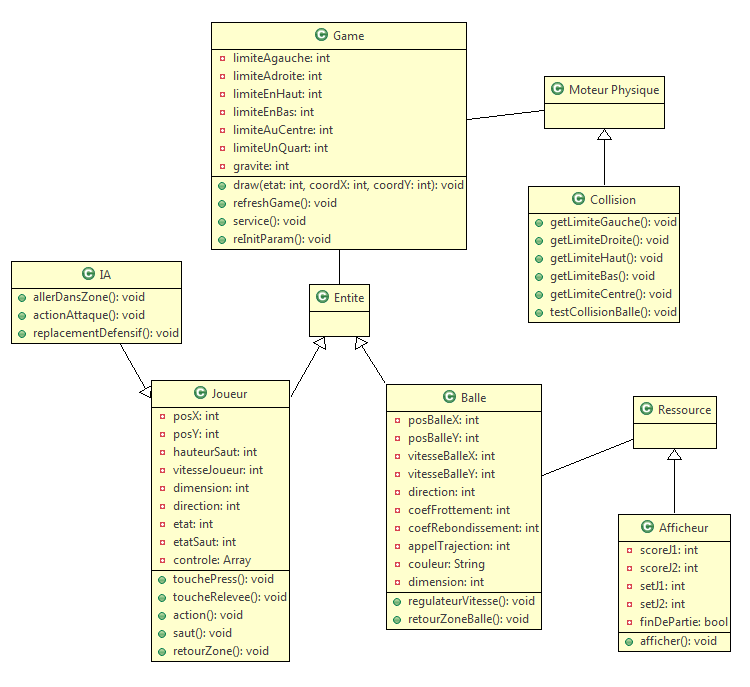
\includegraphics[height=11cm]{../umls/UML_images/Volley/class} \hfill
 \caption{Volley : En haut, diagramme des cas d'utilisation ; en bas, diagramme de classes}
\end{figure}

\begin{figure}[h]
 \centering
 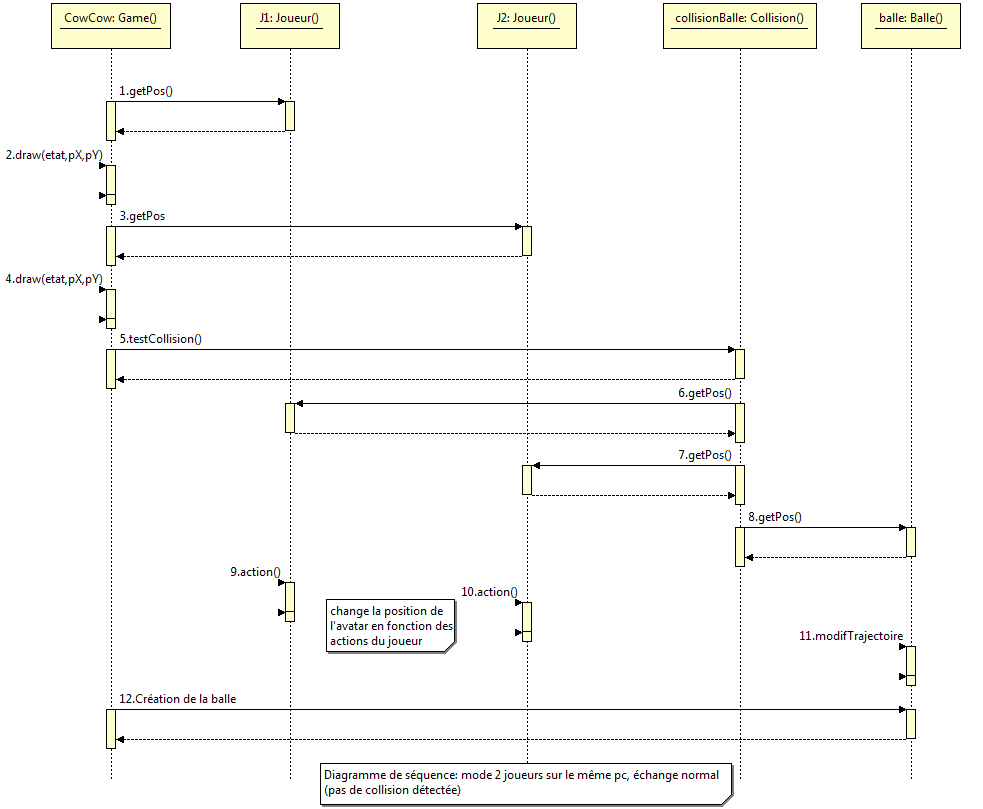
\includegraphics[height=9.5cm]{../umls/UML_images/Volley/sequence} \hfill
 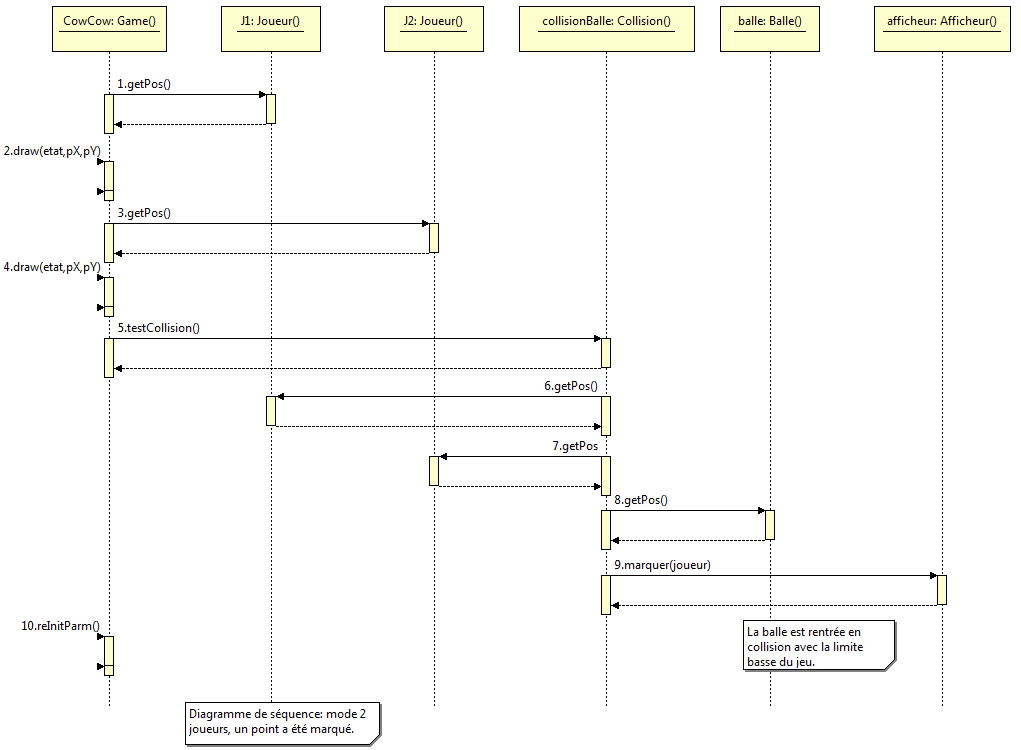
\includegraphics[height=10cm]{../umls/UML_images/Volley/sequence2} \hfill
 \caption{Volley : Diagrammes de séquences}
\end{figure}

% \begin{figure}[h]
%  \centering
%  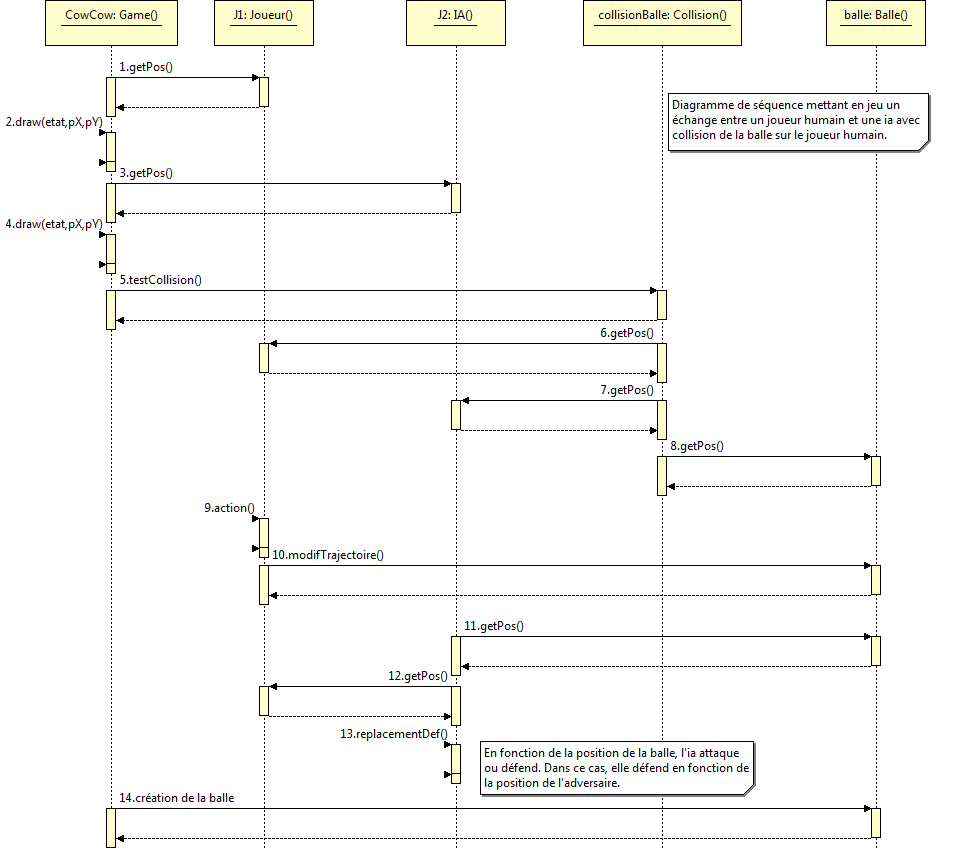
\includegraphics[height=9.5cm]{../umls/UML_images/Volley/sequence3} \hfill
%  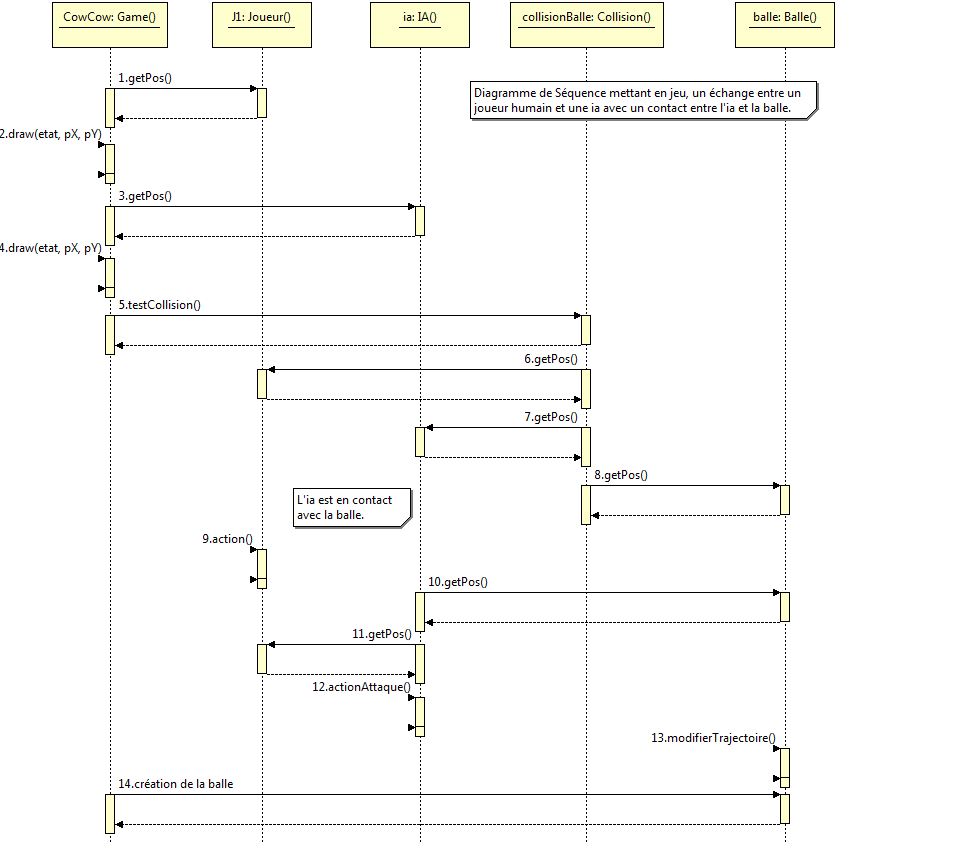
\includegraphics[height=10cm]{../umls/UML_images/Volley/sequence4} \hfill
%  \caption{Volley : D'autres diagrammes de séquences}
% \end{figure}

\clearpage
%% Course

\begin{figure}[h]
 \centering
 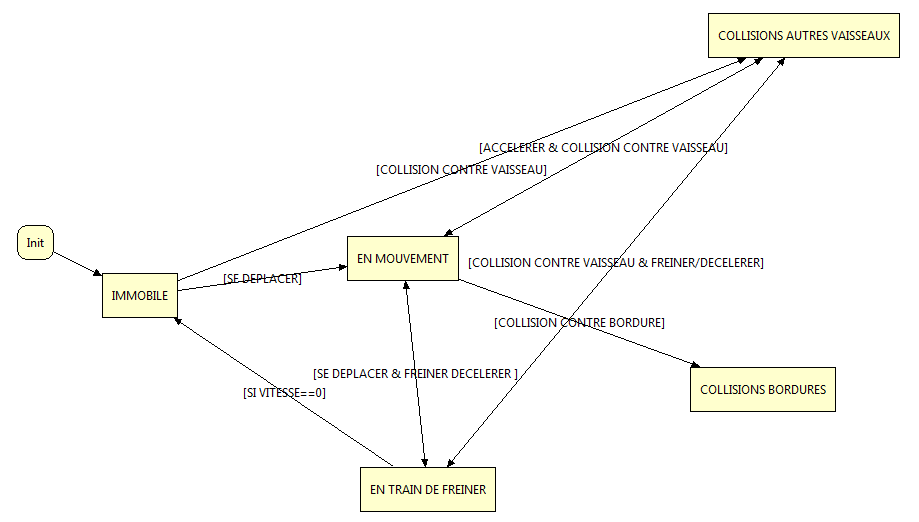
\includegraphics[width=\textwidth,height=9cm]{../umls/UML_images/course/activity} \hfill
 \includegraphics[width=\textwidth]{../umls/UML_images/course/class} \hfill
 \caption{Course : En haut, diagramme d'activité ; en bas, diagramme de classes}
\end{figure}

\begin{figure}[h]
 \centering
 \includegraphics[width=\textwidth]{../umls/UML_images/course/sequence} \hfill
 \caption{Course : Diagramme de séquences}
\end{figure}

\clearpage
%% Mario

\begin{figure}[h]
 \centering
 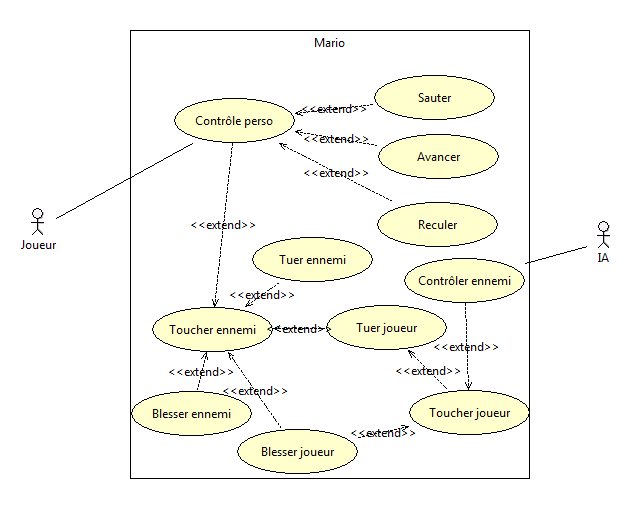
\includegraphics[width=\textwidth]{../umls/UML_images/Mario/Utilisation} \hfill
 \caption{Mario : Diagramme de cas d'utilisation}
\end{figure}

\begin{figure}[h]
 \centering
 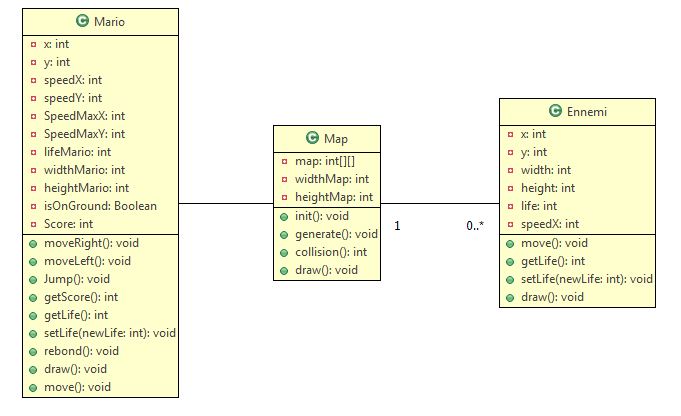
\includegraphics[height=9cm]{../umls/UML_images/Mario/Class} \hfill
 \caption{Mario : Diagramme de classes}
\end{figure}

\begin{figure}[h]
 \centering
 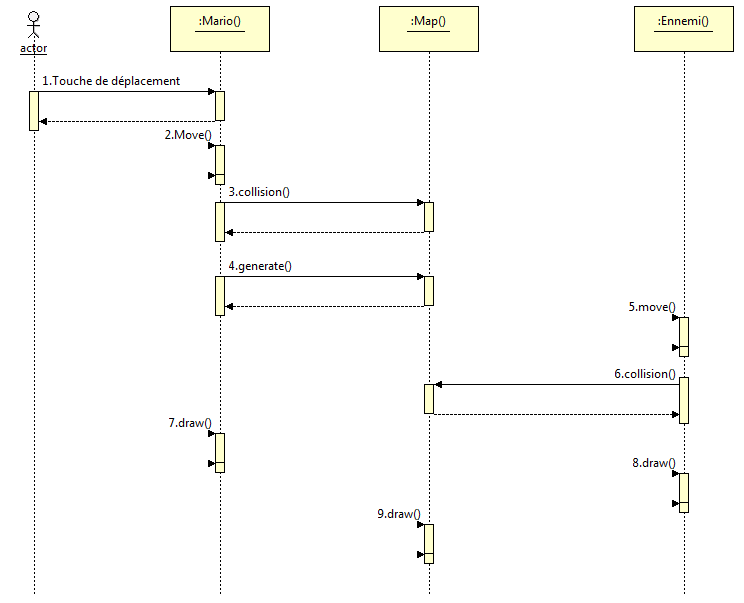
\includegraphics[height=11.5cm]{../umls/UML_images/Mario/Sequence} \hfill
 \caption{Mario : Diagramme de séquences}
\end{figure}


\clearpage
%% WatchNDroid

\begin{figure}[h]
 \centering
 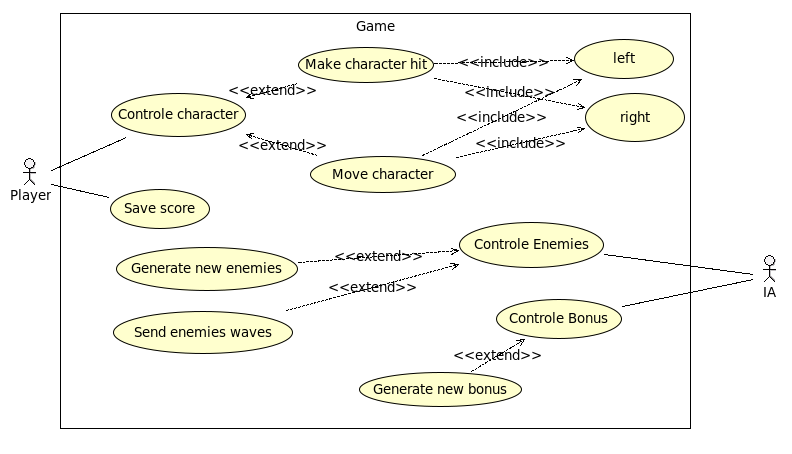
\includegraphics[height=8.5cm]{../umls/UML_images/WatchNDroid/utilisation} \hfill
 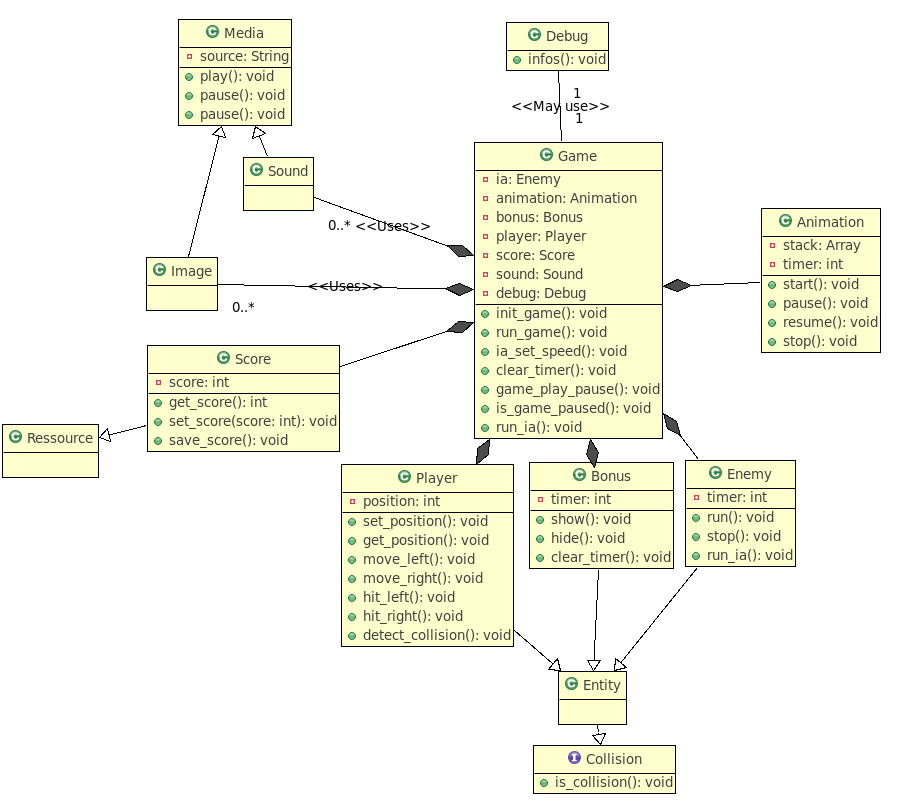
\includegraphics[height=11cm]{../umls/UML_images/WatchNDroid/class} \hfill
 \caption{Watch'N'Droid : En haut, diagramme des cas d'utilisation ; en bas, diagramme de classes}
\end{figure}

\begin{figure}[h]
 \centering
 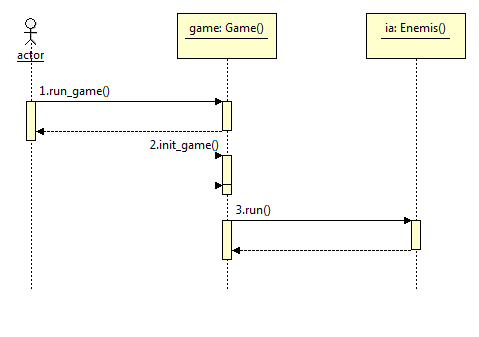
\includegraphics[height=9.5cm]{../umls/UML_images/WatchNDroid/sequence} \hfill
 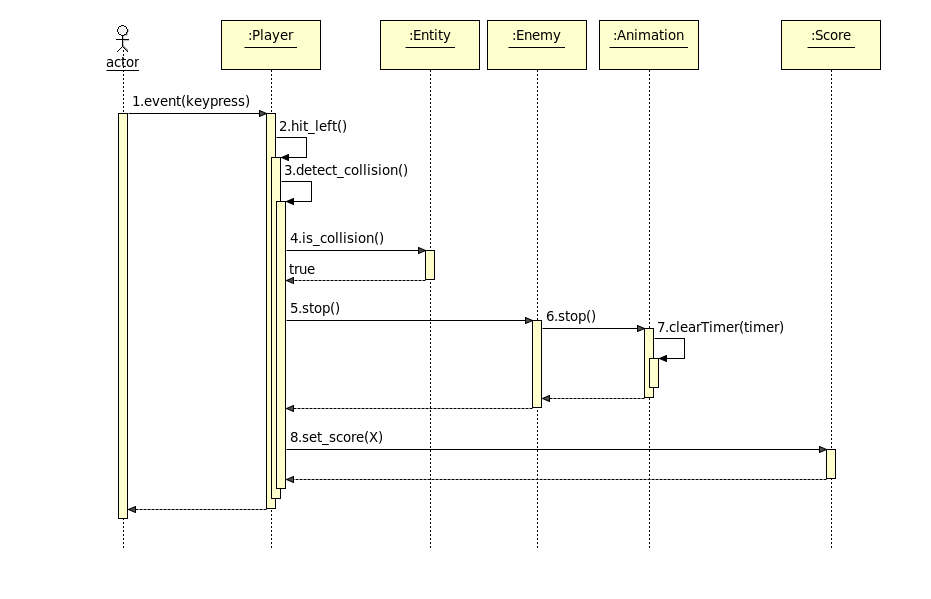
\includegraphics[height=10cm]{../umls/UML_images/WatchNDroid/sequence2} \hfill
 \caption{Watch'N'Droid : Diagrammes de séquences}
\end{figure}

% \begin{figure}[h]
%  \centering
%  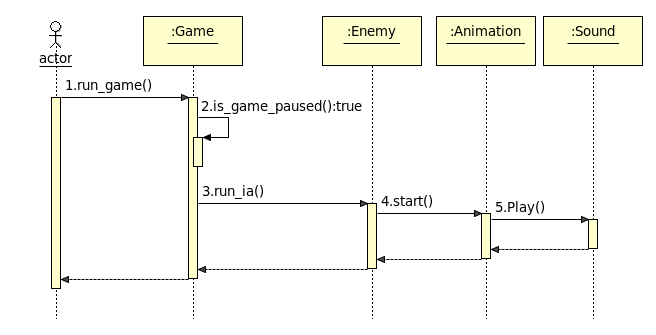
\includegraphics[height=8cm]{../umls/UML_images/WatchNDroid/sequence3} \hfill
%  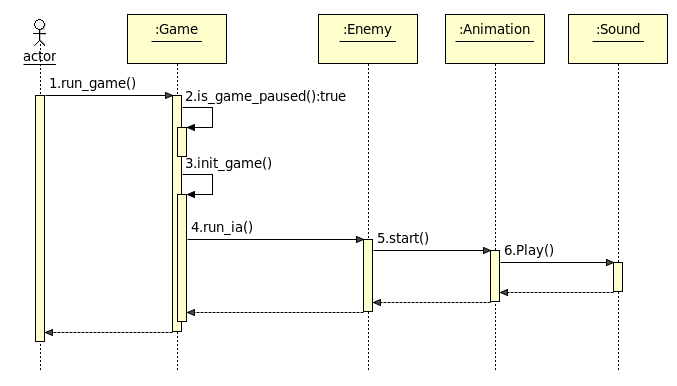
\includegraphics[height=8cm]{../umls/UML_images/WatchNDroid/sequence4} \hfill
%  \caption{Watch'N'Droid : D'autres diagrammes de séquences}
% \end{figure}

\clearpage
%% Billard

\begin{figure}[h]
 \centering
 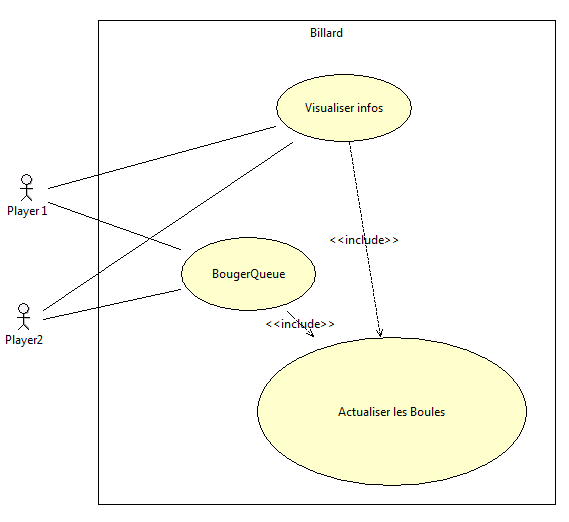
\includegraphics[height=7cm]{../umls/UML_images/Billard/utilisation} \hfill
 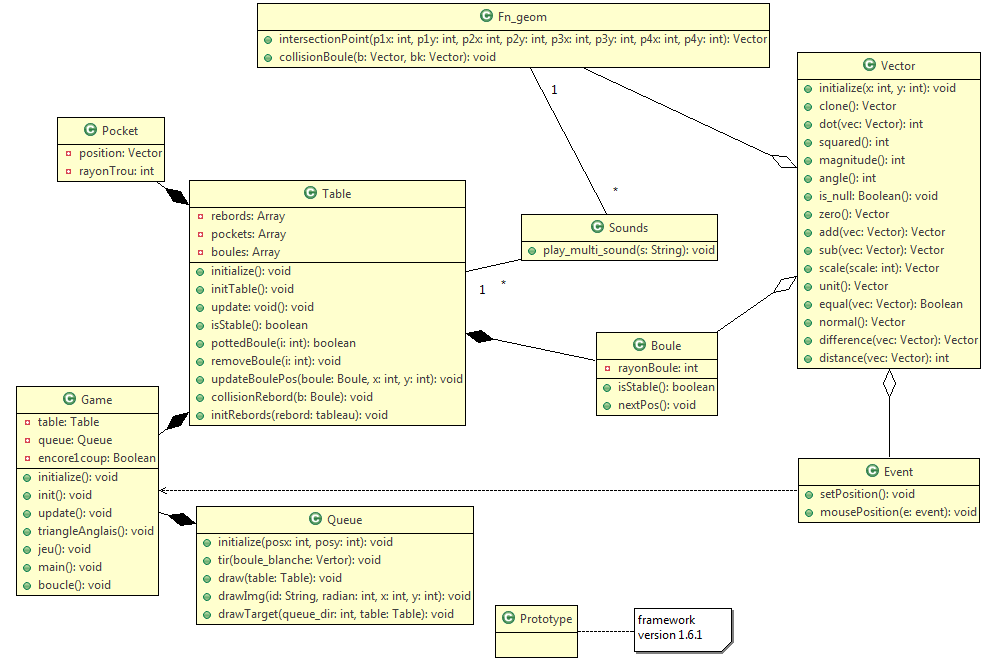
\includegraphics[width=\textwidth,height=12cm]{../umls/UML_images/Billard/class} \hfill
 \caption{Billard : En haut, diagramme des cas d'utilisation ; en bas, diagramme de classes}
\end{figure}

\begin{figure}[h]
 \centering
 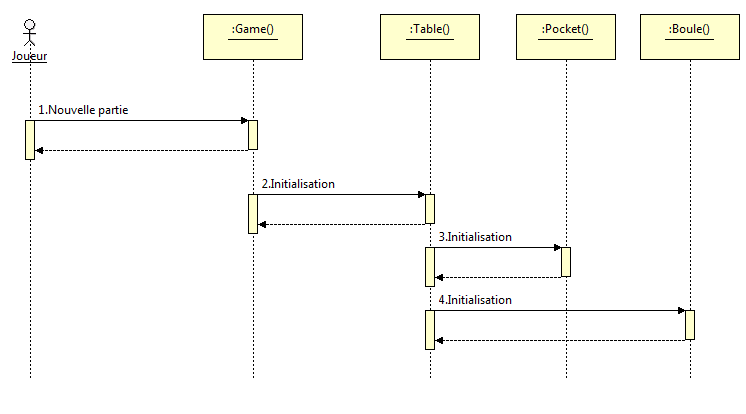
\includegraphics[height=6.5cm]{../umls/UML_images/Billard/sequence1} \hfill
 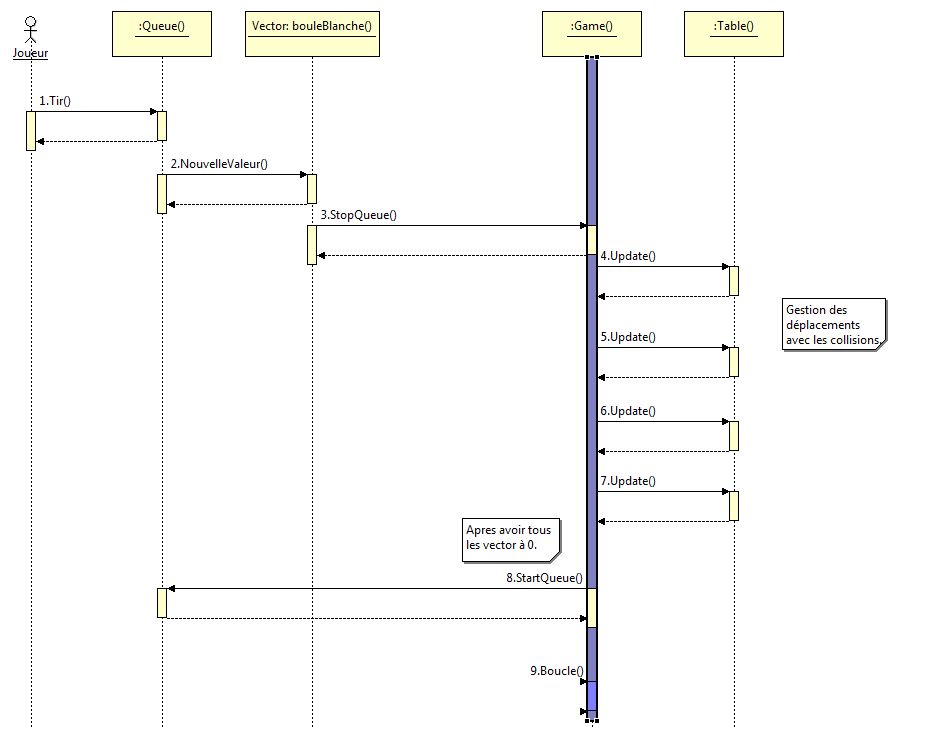
\includegraphics[height=11cm]{../umls/UML_images/Billard/sequence2} \hfill
 \caption{Billard : Diagrammes de séquences}
\end{figure}

\clearpage
%% Commissariat

\begin{figure}[h]
 \centering
 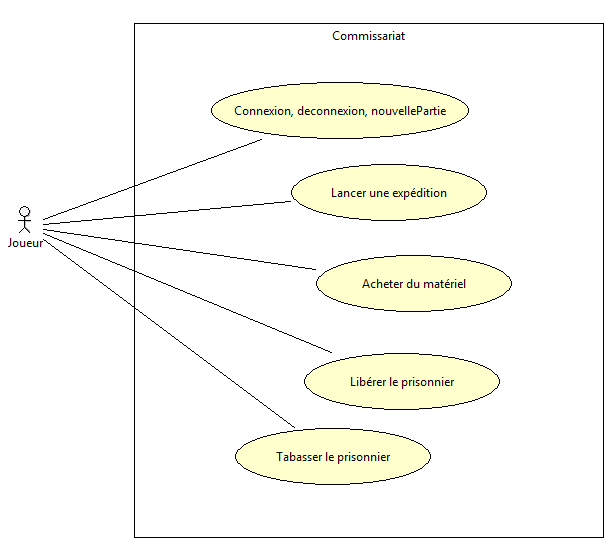
\includegraphics[width=\textwidth]{../umls/UML_images/Commissariat/utilisation} \hfill
 \caption{Gestion : Diagramme de cas d'utilisation}
\end{figure}

\begin{figure}[h]
 \centering
 \includegraphics[width=\textwidth]{../umls/UML_images/Commissariat/class} \hfill
 \caption{Gestion : Diagramme de classes}
\end{figure}
